\chapter{Derived Classes}
\label{chap:derivedClasses}
\section{Inheritance}
\label{sec:inheritance}
Sometimes it is useful to derive new classes from old ones in order to reuse code or to emphasize a program structure. For example, consider the concepts of a \emph{car} and \emph{bicycle}. They are both \emph{vehicles} that can move forward and turn, but a car can move in reverse, has 4 wheels, and uses gasoline or electricity, while a bicycle has 2 wheels and needs to be pedaled. Structurally, we can say that ``a car is a vehicle'' and ``a bicycle is a vehicle''. Such a relation is sometimes drawn as a tree as shown in \Cref{fig:inheritanceVehicle} and is called an \idx{is-a relation}.
%
\begin{figure}
  \centering
  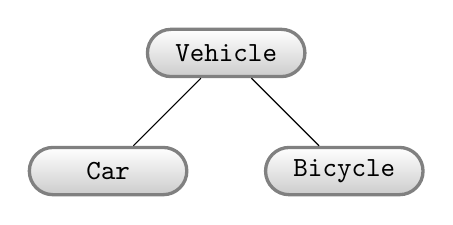
\begin{tikzpicture}[sibling distance=30mm,
    terminal/.style={
      % The shape:
      rectangle,minimum size=6mm,minimum width=20mm,rounded corners=3mm,
      % The rest
      very thick,draw=black!50,
      top color=white,bottom color=black!20,
      font=\ttfamily}]
    \node [terminal] {Vehicle} % root
    child { node [terminal] {Car} }
    child { node [terminal] {Bicycle} };
  \end{tikzpicture}
  \caption{Both a car and a bicycle is a (type of) vehicle.}
  \label{fig:inheritanceVehicle}
\end{figure}
%
Is-a relations can be implemented using class \idx{inheritance}, where vehicle is called the \idx{base class}, and car and bicycle are each a \idx{derived class}. The advantage is that a derived class can inherent the members of the base class, \idx{override}, and possibly add new members. Another advantage is that objects from derived classes can be made to look like as if they were objects of the base class while still containing all their data. Such mascarading is useful when, for example, listing cars and bicycles in the same list.

In F\#, inheritance is indicated using the \lstinline[language=syntax]{inherit} keyword in the class definition. An extensions of the syntax in \Cref{\ebnf/class.ebnf} is:
%
\begin{verbatimwrite}{\ebnf/class.ebnf}
type <*classIdent*> ({*<*arg*>*}) [*as <*selfIdent*>*] 
  [*inherit <*baseClassIdent*>({*<*arg*>*})*]
  {*[*let <*binding*>*] |* [*do <*statement*>*]*}
  {*(*member |* abstract member |* default |* override*) <*memberDef*>*}
\end{verbatimwrite}
\syntax{\ebnf/class.ebnf}{A class definition with inheritance.}
%
New syntactical elements are: the  \lstinline{inherit} keyword, which indicates that this is a derived class and where \lstinline[language=syntax]{<*baseClassIdent*>} is the name of the base class. Further, members may be regular members using the \lstinline{member} keyword as discussed in the previous chapter, and members can also be other types, as indicated by the keywords: \lstinline{abstract member}, \lstinline{default}, and \lstinline{override}.

An example of defining base and derived classes for vehicles is shown In \Cref{vehicle}.
%
%\fs{classInheritance}{New classes can be derived from old.}
\fs{vehicle}{New classes can be derived from old ones.}
%
In the example, a simple base class \lstinline{vehicle} is defined to include \lstinline{wheels} as its single member. The derived classes inherit all the members of the base class, but do not have access to any non-members of the base constructor. I.e., \lstinline{car} and \lstinline{bicycle} automatically have the \lstinline{wheels} attribute. Both derived classes additional members \lstinline{maxPassengers} and \lstinline{mustUseHelmet}, respectively.

Derived classes can replace base class members by defining new members \idx{overshadow} the base members. The base members are still available through the \idx[base@\lstinline{base}]{\keyword{base}}-keyword. Consider the example in the \Cref{memberOvershadowing}.
%
\fs{memberOvershadowing}{Inherited members can be overshadowed, but we can still access the base member.}
%
In this case, we have defined two counters, each with an internal field \lstinline{i} and with members \lstinline{value} and \lstinline{inc}. The \lstinline{inc} method in \lstinline{counter} increments \lstinline{i} with 1, and in \lstinline{counter2} the field \lstinline{i} is incremented with 2. Note how \lstinline{counter2} inherits both members \lstinline{value} and \lstinline{inc}, but overshadows \lstinline{inc} by defining its own. Note also how \lstinline{counter2} defines another method \lstinline{incByOne} by accessing the inherited \lstinline{inc} method using the \keyword{base} keyword.

Even though derived classes are different from their base, the derived class includes the base class, which can be recalled using \idx[upcast]{upcasting} by the upcast operator \idx[:>@\lstinline{:>}]{\lexeme{:>}}. At compile-time, this operator removes the additions and overshadowing of the derived class, as illustrated in \Cref{upCasting}. 
%
\fs{upCasting}{Objects can be upcasted resulting in an object to appear to be of the base type. Implementations from the derived class are ignored.}
%
Here \lstinline{howdy} is derived from \lstinline{hello}, overshadows \lstinline{str}, and adds property \lstinline{altStr}. By upcasting object \lstinline{b}, we create object \lstinline{c} as a copy of \lstinline{b} with all its fields, functions, and members, as if it had been of type \lstinline{hello}. I.e., \lstinline{c} contains the base class version of \lstinline{str} and does not have property \lstinline{altStr}. Objects \lstinline{a} and \lstinline{c} are now of same type and can be put into, e.g., an array as \lstinline{let arr = [|a, c|]}. Previously upcasted objects can also be downcasted again using the \idx{downcast} operator \idx[:?>@\lstinline{:?>}]{\keyword{:?>}}, but the validity of the operation is checked at runtime. Thus, \advice{avoid downcasting when possible.}

\section{Interfacing with the \lstinline{printf} Family}
In previous examples, we accessed the property in order to print the contents of objects. Luckily, a more elegant solution is available. Objects can be printed directly, but the result is most often not very useful, as can be seen in \Cref{classPrintf}.
%
\fs [linebackgroundcolor={%
\highlight{\getrefnumber{classPrintfApp}}%
}]{classPrintf}{Printing classes yields low-level information about the class.}
%
All classes are given default members through a process called \idx{inheritance}, to be discussed below in \Cref{sec:inheritance}. One example is the \lstinline{ToString() : () -> string} function, which is useful in conjunction with, e.g., \lstinline{printf}. When an object is given as argument to a \lstinline{printf} function, then \lstinline{printf} calls the object's \lstinline{ToString()} function. The default implementation returns low-level information about the object, as can be seen above, but we may \idx{override}
 this member using the \idx{\keyword{override}}-keyword, as demonstrated in \Cref{classToString}.\jon{something about ToString not working with 's' format string in printf.}
%
\fs[linebackgroundcolor={%
\highlightRange{\getrefnumber{classToStringStart}}{\getrefnumber{classToStringEnd}}%
\highlight{\getrefnumber{classToStringApp}}%
}]{classToString}{Overriding \lstinline{ToString()} function for better interaction with members of the \lstinline{printf} family of procedures.  Compare with \Cref{classPrintf}.}
%
We see that as a consequence, the \lstinline{printf} statement is much simpler. However beware, an application program may require other formatting choices than selected at the time of designing the class, e.g., in our example, the application program may prefer square brackets as delimiters for vector tuples.  So in general \advice{when designing an override to \lstinline{ToString()}, choose simple, generic formatting for the widest possible use.} 

The most generic formatting is not always obvious, and in the vector case some candidates for the formatting string of \lstinline{ToString()} are ``\lstinline{%A %A}'', ``\lstinline{%A, %A}'', ``\lstinline{(%A, %A)}'', and ``\lstinline{[%A, %A]}''.
 Considering each carefully, it seems that arguments can be made against all them. A common choice is to let the formatting be controlled by static members that can be changed by the application program through accessors.

\section{Abstract Classes}
\label{sec:abstract}
In the previous sections, we have discussed inheritance as a method to modify and extend any class. I.e., the definition of the base classes were independent of the definitions of inherited classes. In that sense, the base classes were oblivious to any future derivation of them. Sometimes it is useful to define base classes which are not independent of derived classes and which impose design constraints of derived classes. Two such dependencies in F\# are abstract classes and interfaces.

 An \idx{abstract class} contains members defined using the \idx[abstract member@\lstinline{abstract member}]{\lstinline{abstract member}} and optionally the \idx[default@\lstinline{default}]{\lstinline{default}} keywords. An \lstinline{abstract member} in the base class is a type definition, and derived classes must provide an implementation using the \idx[override@\lstinline{override}]{\keyword{override}} keyword. Optionally, the base class may provide a default implementation using the \lstinline{default} keyword, in which case overriding is not required in derived classes. Objects of classes containing abstract members without default implementations cannot be instantiated, but derived classes that provide the missing implementations can. Note that abstract classes must be given the \idx[AbstractClass@\lstinline{[<AbstractClass>]}]{\lstinline{[<AbstractClass>]}} attribute. Note also that in contrast to overshadowing, upcasting keeps the implementations of the derived classes. Examples of this are shown in \Cref{abstractClass}.
%
\fs{abstractClass}{In contrast to regular objects, upcasted derived objects use the derived implementation of abstract methods.}
%
In the example, we define a base class and two derived classes. Note how the abstract member is defined in the base class using the \lexeme{:}-operator as a type declaration rather than a name binding. Note also that since the base class does not provide a default implementation, the derived classes supply an implementation using the \keyword{override}-keyword. In the example, objects of \lstinline{baseClass} cannot be created, since such objects would have no implementation for \lstinline{this.hello}. Finally, the two different derived and upcasted objects can be put in the same array, and when calling their implementation of \lstinline{this.hello}, we still get the derived implementations, which is in contrast to overshadowing.

Abstract classes may also specify a default implementation, such that derived classes have the option of implementing an overriding member, but are not forced to. In spite of implementations being available in the abstract class, the abstract class still cannot be used to instantiate objects. The example in \Cref{abstractDefaultClass} shows an extension of \Cref{abstractClass} with a default implementation.
%
\fs[linebackgroundcolor={%
\highlightRange{\getrefnumber{abstractDefaultClassStart}}{\getrefnumber{abstractDefaultClassEnd}}%
}]{abstractDefaultClass}{Default implementations in abstract classes make implementations in derived classes optional. Compare with \Cref{abstractClass}.}%
%
In the example, the program in \Cref{abstractClass} has been modified such that \lstinline{greeting} is given a default implementation for \lstinline{str}, in which case \lstinline{hello} does not need to supply one. However, in order for \lstinline{howdy} to provide a different greeting, it still needs to provide an override member. 

Note that even if all abstract members in an abstract class have defaults, objects of its type can still not be created, but must be derived as, e.g., shown with \lstinline{hello} above.

As a side note, every class implicitly derives from a base class \idx[System.Object@\lstinline{System.Object}]{\lstinline{System.Object}}, which is an abstract class defining among other members, the \lstinline{ToString} method with default implementation.

\section{Interfaces}
\label{sec:interfaces}
Inheritance of an abstract base class allows an application to rely on the definition of the base, regardless of any future derived classes. This gives great flexibility, but at times even less knowledge is needed about objects in order to write useful applications. This is what \idx[interface]{interfaces} offer. An interface specifies which members must exist, but nothing more. Interfaces are defined as an abstract class \emph{without arguments} and \emph{only with abstract members}. Classes implementing interfaces must specify implementations for the abstract members using the \idx[interface with@\lstinline{interface with}]{\lstinline{interface with}} keywords. Objects of classes implementing interfaces can be upcasted as if they had an abstract base class of the interface's name. Consider the example in \Cref{classInterface}.
%
\fs{classInterface}{Interfaces specify which members classes contain, and with upcasting gives more flexibility than abstract classes.}
%
Here, two distinctly different classes are defined: \lstinline{house} and \lstinline{person}. These are not related by inheritance, since no sensible common structure seems available. However, they share structures in the sense that they both have an integer property and a \lstinline{float -> float} method. For each of the derived classes, these members have different meanings. Still, some treatment of these members by an application will only rely on their type and not their meaning. E.g., in \Cref{classInterface}, the \lstinline{printfn} function only needs to know the member's type, not its meaning. As a consequence, the application can upcast them both to the implicit abstract base class \lstinline{IValue}, put them in an array, and apply a function using the member definition of \lstinline{IValue} with the higher-order \lstinline{List.iter} function. Another example could be a higher-order function calculating average values: For average values of the number of floors and average value of the length of people's names, the higher-order function would only need to know that both of these classes implement the \lstinline{IValue} interfaces in order to calculate the average of list of either objects' types.

As a final note, inheritance ties classes together in a class hierarchy. Abstract members enforce inheritance and impose constraints on the derived classes. Like abstract classes, interfaces impose constraints on derived classes, but without requiring a hierarchical structure.

\section{Programming Intermezzo: Chess}
To demonstrate the use of hierarchies, consider the following problem.
\begin{problem}
  The game of chess is a turn-based game for two which consists of a board of $8\times 8$ squares, and a set of 16 black and 16 white pieces. A piece can be either a king, queen, rook, bishop, knight or pawn, and each piece has a specific movement pattern on the board. Pieces are added to, moved on, and removed from the board during the game, and there can be at most one piece per square. A piece strikes another piece of opposing color by moving to its square and the piece of opposing color is removed from the game. The game starts with the configuration shown in \Cref{fig:chessNewGame}.\\[\parskip]

  Make a program that allows two humans to play simple chess using only kings and rooks. The king must be able to move to all neighboring squares not occupied by a piece of the same color and cannot move onto a square where it can be struck in the next turn. The rook must be able to move in horizontal and vertical lines until a piece of the same color or up to and including a piece of opposing color.
\end{problem}
\begin{figure}
  \centering
  \newgame
  \showboard
  \caption{Starting position for the game of chess.}
  \label{fig:chessNewGame}
\end{figure}
Since we expect that the solution to the above problem is going to be a relatively long program, we have decided to split the code into a library and an application program. Before writing a library, it is often useful to start thinking about how the library should be used. Thus we start by sketching the application program, and in the process consider options for the main methods and properties to be used.

We also foresee future extensions to include more pieces, but also that these pieces will obey the same game mechanics that we design for the present problem. Thus, we will put the main part of the library in a file defining the module called \lstinline{Chess} and the derived pieces in another file defining the module \lstinline{Pieces}.

%For a solution, the application must be able to create pieces of various types and colors, to set, move and remove pieces position, and to acquire a piece's location on the board, if it is still in the game. 
%
Every game needs a board, and we will define a class \lstinline{Board}. A board is like an array, so it seems useful to be able to move pieces by index notation. Thus, the board must have a two-dimensional \lstinline{Item} property. We also decide that each position will hold an option type, such that when a square is empty it holds \lstinline{None}, and otherwise it holds piece \lstinline{p} as \lstinline{Some p}. Although chess notation would be neat, for ease of programming we will let index (0,0) correspond to position a1 in chess notation, etc. The most common operation will probably be to move pieces around, so we will give the board a \lstinline{move} method. We will most likely also like to print the board with pieces in their right locations. For simplicity, we choose to override the \lstinline{ToString} method in \lstinline{Board}, and that this method also prints information about each individual piece, such as where it is, where it can move to, and which pieces it can either protect or hit. The pieces that a piece can protect or hit we will call the piece's neighbor pieces.

A piece can be one of several types, so this gives a natural hierarchical structure which is well suited for inheritance. Each piece must be given a color, which may conveniently be given as argument at instantiation. Thus, we have decided to make a base class called \lstinline{chessPiece} with argument \lstinline{Color}, and derived classes \lstinline{king} and \lstinline{rook}. The color may conveniently be define as a discriminated union type of either \lstinline{White} or \lstinline{Black}. Each piece will also override the \lstinline{ToString} method for ease of printing. The override will be used in conjunction with the board's override, so it should only give information about the piece's type and color. For compact printing, we will use a single letter for the type of piece, upper case if white, and lower case if black. We expect the pieces also to need to know something about the their relation to board, so we will make a \lstinline{position} property which holds the coordinates of the piece, and we will make a \lstinline{availableMoves} method that lists the possible moves a piece can make. Thus, we produce the application in \Cref{chessAppCode}, and an illustration of what the program should do is shown in \Cref{fig:chessKingsGame}.
%
\fsCode{chessApp}{chessAppCode}{A chess application.}{}
%
\begin{figure}
  \centering
  \newgame
  \loadgame{figures/kingsGame}
  \showboard
  \hspace*{1cm}
  \loadgame{figures/kingsGameMove}
  \showboard
  \caption{Starting at the left and moving white rook to b4.}
  \label{fig:chessKingsGame}
\end{figure}
At this point, we are fairly happy with the way the application is written. The double bookkeeping of pieces in an array and on the board seems a bit excessive, but for testing it seems useful to be able to easily access all pieces, both those in play and struck. Although the \lstinline{position} property of a \lstinline{chessPiece} could be replaced by a function searching for a specific piece on the board, we have a hunch that we will need to retrieve a piece's position often, and that this double bookkeeping will most likely save execution time later. 

Continuing our outer to inner approach, as a second step, we consider the specific pieces: They will inherit a base piece and implement the details that are special for that piece. Each piece is signified by its color and its type, and each type has a specific motion pattern. Since we have already decided to use discriminated unions for the color, it seems natural to let the color be part of the constructor of the base class. As in the example application in \Cref{chessAppCode}, pieces are upcasted to \lstinline{chessPiece}, thus, the base class must know how to print the piece type. For this, we will define an abstract property, such that everything needed for overriding \lstinline{ToString} is available to the base class, but also such that the name of the type of the piece is set in the derived class.

For a piece on the board, its available moves depend on its type and the other pieces. The application program will need to make a decision on whether to move the piece depending on which vacant squares it can move to, and its relation to its neighbors, i.e., is the piece protecting one of its own color, or does it have the opportunity to hit an opponent's piece. Thus, given the board with all the pieces, it seems useful that \lstinline{availableMoves} returns two lists: a list of vacant squares and a list of neighboring pieces of either color. Each piece has a certain movement pattern which we will specify regardless of the piece' position on the board and relation to other pieces. Thus, this will be an abstract member called \lstinline{candidateRelativeMoves} implemented in the derived pieces. These candidate relative moves are then to be sifted for legal moves, and the process will be the same for all pieces. Thus sifting can be implemented in the base class as the \lstinline{availableMoves}.

Many pieces move in runs, e.g., the rook can move horizontally and vertically until there is another piece. Vacant squares behind the blocking piece are unavailable. For a rook, we thus must analyze four runs: northward, eastward, southward, and westward. For each run, we must consult the board to see how many vacant fields there are in that direction, and which is the piece blocking, if any. Thus, we decide that the board must have a function that can analyze a list of runs, and that the result is concatenated into a single list of vacant squares and a single list of neighboring pieces, if any. This function we call \lstinline{getVacentNNeighbours}. And so we arrive at \Cref{pieces}.
%
\fsImplementation{pieces}{pieces}{An extension of chess base.}{}
%
The king has the simplest relative movement candidates, being the hypothetical eight neighboring squares. For rooks, the relative movement candidates are somewhat more complicated. For rooks, we would like to use \lstinline{List.map} to convert a list of single indices into double indices to calculate each run. For this, we have gathered all the elemental functions in \lstinline{indToRel}. E.g., for the function at index 0, we may write \lstinline{List.map indToRel.[0] indices}. However, we would also like to use \lstinline{List.map} to perform this operation for all elemental functions in \lstinline{indToRel}. Direct joining such two applications of \lstinline{List.map} does not work, since \lstinline{List.map} takes a function and a list as its arguments, and for the second application, these two arguments should switch order.  I.e., the first time it is \lstinline{indices} that takes the role of the list, while the second it is \lstinline{indToRel} that takes the role of the list. A standard solution in functional programming is to use currying and the \idx{\lstinline{swap}} function, as illustrated in line~\ref{chessPieceSwapApp}: The function is equivalent to the anonymous function \lstinline{fun elm -> swap List.map indices elm}, and since \lstinline{swap} swaps the arguments of a function, this reduces to \lstinline{fun elm -> List.map elm indices}, which is exactly what is needed.

The final step will be to design the \lstinline{Board} and \lstinline{chessPiece} classes. The Chess module implements discriminated unions for color and an integer tuple for a position. These are shown in \Cref{chessDiscriminatedUniont}.
%
\fsImplementation{chess}{chessDiscriminatedUniont}{A chess base: Module header and discriminated union types.}{lastline=3}
%
The \lstinline{chessPiece} will need to know what a board is, so we must define it as a mutually recursive class with \lstinline{Board}. Furthermore, since all pieces must supply an implementation of \lstinline{availableMoves}, we set it to be abstract by the abstract class attribute and with an abstract member. The board will need to be able to ask for a string describing each piece, and to keep the board on the screen we include an abbreviated description of the piece's properties color and piece type. The result is shown in \Cref{chessPiece}.
%
\fsImplementation{chess}{chessPiece}{A chess base. Abstract type chessPiece.}{firstnumber=4,firstline=4,lastline=24} % Absolute reference!
%

Our \lstinline{Board} class is by far the largest and will be discussed in \Crefrange{chessBoardConstructor}{chessBoardgetVacantNOccupied}. The constructor is shown in \Cref{chessBoardConstructor}.
%
\fsImplementation{chess}{chessBoardConstructor}{A chess base: the constructor}{firstnumber=25,firstline=25,lastline=42} % Absolute reference!
%
For memory efficiency, the board has been implemented using a \lstinline{Array2D}, since pieces will move around often. For later use, in the members shown in \Cref{chessBoardgetVacantNOccupied} we define two functions that convert relative coordinates into absolute coordinates on the board, and remove those that fall outside the board. These are called \lstinline{validPositionWrap} and \lstinline{relativeToAbsolute}.

For ease of use in an application, \lstinline{Board} implements \lstinline{Item}, such that the board can be read and written to using array notation. And \lstinline{ToString} is overridden, such that an application may print the board anytime using a \lstinline{printf} function. This is shown in \Cref{chessBoardItem}.
%
\fsImplementation{chess}{chessBoardItem}{A chess base: Board header, constructor, and non-static members.}{firstnumber=43,firstline=43,lastline=73} % Absolute reference!
%
Note that for efficiency, location is also stored in each piece, so \lstinline{set} also needs to update the particular piece's position, as done in line~\ref{chessItemSet}. Note also that the board is printed with the first coordinate of the board being rows and second columns, and such that element (0,0) is at the bottom right complying with standard chess notation.

The main computations are done in the static methods of the board, as shown in \Cref{chessBoardgetVacantNOccupied}. 
%
\fsImplementation{chess}{chessBoardgetVacantNOccupied}{A chess base: Board static members.}{firstnumber=74,firstline=74} % Absolute reference!
%
A chess piece must implement \lstinline{candiateRelativeMoves}, and we decided in \Cref{chessPiece} that moves should be specified relative to the piece's position. Since the piece does not know which other pieces are on the board, it can only specify all potential positions. For convenience, we will allow pieces to also specify positions outside the board, such that, e.g., the rook can specify the 7 nearest neighboring squares up, down, left, and right, regardless that some may be outside the board. Thus \lstinline{getVacantNNeighbours} must first convert the relative positions to absolute and clip any outside the board. This is done by \lstinline{relativeToAbsolute}. Then for each run, the first occupied square must be identified. Since \lstinline{availableMoves} must return two lists, vacant squares, and immediate neighbors, this structure is imposed on the output of \lstinline{convertNWrap} as well. This is computed in \lstinline{getVacantNOccupied} by use of the built-in \lstinline{List.findIndex} function. This function returns the index of the first element in a list for which the supplied function is true and otherwise throws an exception. Exceptions are always somewhat inelegant, but in this case, it is harmless, since the exception signifies a valid situation where no pieces exist on the run. After having analyzed all runs independently, then all the vacant lists are merged, all the neighboring pieces are merged and both are returned to the caller.

Compiling the library files with the application and executing gives the result shown in \Cref{chessApp}.
%
\fsOutput{chessApp}{Running the program. Compare with \Cref{fig:chessKingsGame}.}{}
%
We see that the program has correctly determined that initially, the white king has the white rook as its neighbors and due to its location in the corner only has two free positions to move to. The white rook has many and the black king as its neighbor. The black king is free to move to all its eight neighboring fields. After moving the white rook to (3,1) or b4 in regular chess notation, then the white king has no neighbors, and the white rook and the black king are now neighbors with an appropriate restriction on their respective vacant squares. These simple use-tests are in no way a thorough test of the quality of the code, but they give us a good indication that our library offers a tolerable interface for the application, and that at least major parts of the code function as expected. Thus, we conclude this intermezzo.

%%% Local Variables:
%%% TeX-master: "fsharpNotes"
%%% End:

